\section{MWCモデル}

ヘモグロビンと酸素の結合を記述する有力なモデルとして,KNF(Koshland, N\'{e}methy, Filmer)モデルとMWC(Monod, Wyman, Changeux)モデルが知られている.
これらのモデルでは,Hillの式で無視されていた,受容体(ヘモグロビン)のサイトの一部にだけリガンド(酸素)が結合した状態も含めて取り扱う.
ここではとくにMWCモデルを紹介する.

\subsection{準備}

\begin{figure}[htbp]
  \centering
  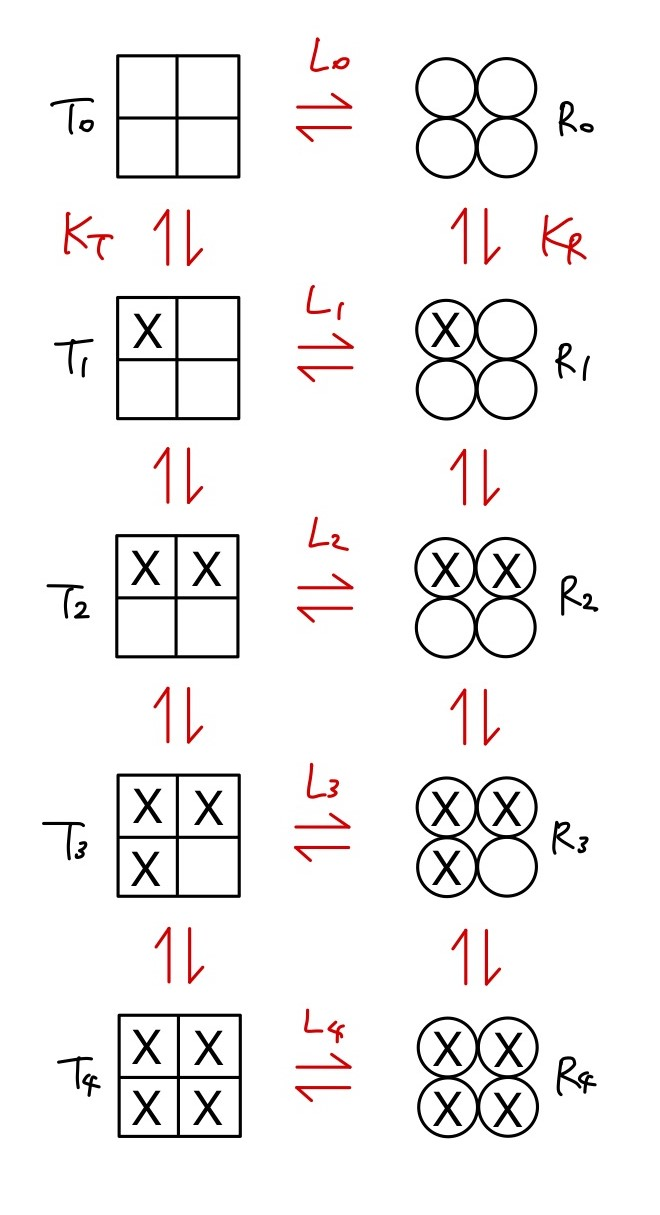
\includegraphics[width=5cm]{mwc_scheme.jpg}
  \caption{MWCモデルの概略図}
  \label{fig:mwc_scheme}
\end{figure}

MWCモデルでは,受容体が$n$個のサブユニットからなり,それぞれのサブユニットに一つずつリガンド結合サイトがあると考える.(ヘモグロビンと酸素の結合を考える際は$n=4$である.)
さらに,受容体が二つの状態(tense状態とrelaxed状態.それぞれT,Rと表す)の間を遷移すると考える\footnote{最近の研究ではヘモグロビンの状態としてT,Rの他にR2というものも見つかっており,実際のヘモグロビンの挙動はもっと複雑であると考えられている\cite{review}.}.
T状態の受容体に$i$個のリガンドが結合した状態を$\ce{T_{$i$}}$,R状態の受容体に$i$個のリガンドが結合した状態を$\ce{R_{$i$}}$と書く.
また,T(R)状態の受容体の空きサイトにリガンドが結合する反応の速度定数は$k_{\mathrm{on},\ce{T}}$($k_{\mathrm{on},\ce{R}}$),その逆反応は$k_{\mathrm{off},\ce{T}}$($k_{\mathrm{off},\ce{R}}$)で一定とする.
このとき,各反応の会合定数(解離定数の逆数)は
\begin{equation}
  K_{\ce{T}} = \frac{k_{\mathrm{on},\ce{T}}}{k_{\mathrm{off},\ce{T}}} \qquad K_{\ce{R}} = \frac{k_{\mathrm{on},\ce{R}}}{k_{\mathrm{off},\ce{R}}}
\end{equation}
となる(図\ref{fig:mwc_scheme}).

また,$n$個のサブユニットを区別し,どのような順番でもリガンドが結合できると仮定する.
たとえばリガンドが1つだけ結合した$\ce{T1}$は,実際には「どのサブユニットにリガンドが結合しているか」によって区別された$n$通りの状態を含むと考える.
これをもとに,$i=1,2,\cdots,n$に対して$\ce{T_$i-1$}$と$\ce{T_$i$}$の間の遷移を考える.
まず$\ce{T_$i-1$}$から$\ce{T_$i$}$への反応は,リガンドの結合していない$n-i+1$個のサイトで起こるので,速度定数は$(n-i+1)k_{\mathrm{on},\ce{T}}$となる.
一方でその逆反応は,リガンドの結合している$i$個のサイトで起こるので,速度定数は$ik_{\mathrm{off},\ce{T}}$となる.
$\ce{R_$i-1$}$と$\ce{R_$i$}$の間の遷移についても同様のことがいえる.

先ほどまではレート方程式を立てて定常状態を議論したが,ここでは簡単のため,すべての反応について化学平衡が成り立つと考えて平衡状態を議論する.
そのため,次が成り立つと考える:
\begin{align}
  (n-i+1)k_{\mathrm{on},\ce{T}}[\ce{T_$i-1$}][\ce{X}] &= ik_{\mathrm{off},\ce{T}}[\ce{T_$i$}] \\
  (n-i+1)k_{\mathrm{on},\ce{R}}[\ce{R_$i-1$}][\ce{X}] &= ik_{\mathrm{off},\ce{R}}[\ce{R_$i$}]
\end{align}
これより,
\begin{align}
  [\ce{T_$i$}] &= {}_n \mathrm{C}_i (K_{\ce{T}}[\ce{X}])^i [\ce{T0}] \label{Ti}\\
  [\ce{R_$i$}] &= {}_n \mathrm{C}_i (K_{\ce{R}}[\ce{X}])^i [\ce{R0}] \label{Ri}
\end{align}
がいえる.
加えて,すべての反応が平衡にあると考えるので,$\ce{T_$i$}$と$\ce{R_$i$}$の間の平衡も考える必要がある.
$\ce{T_$i$}$から$\ce{R_$i$}$への反応の速度定数を$l_{\ce{TR},i}$,その逆反応の速度定数を$l_{\ce{RT},i}$とおく.
このとき,この間の平衡定数を
\begin{equation}
  L_{i} = \frac{l_{\ce{RT},i}}{l_{\ce{TR},i}} = \frac{[\ce{T_$i$}]}{[\ce{R_$i$}]} \label{Li_def}
\end{equation}
とおく.

ただし,今まで考えてきた「すべての反応が平衡」という状況が実現するには条件がある.
それは,式\eqref{Li_def}に式\eqref{Ti}と式\eqref{Ri}を代入すると得られる式
\begin{equation}
  L_{i} = \frac{{}_n \mathrm{C}_i (K_{\ce{T}}[\ce{X}])^i [\ce{T0}]}{{}_n \mathrm{C}_i (K_{\ce{R}}[\ce{X}])^i [\ce{R0}]} = L_0 c^i \label{Li}
\end{equation}
である.ここで,
\begin{equation}
  c = \frac{K_{\ce{T}}}{K_{\ce{R}}}
\end{equation}
とおいた.
平衡定数$L_i$がこれを満たさないと3つの式\eqref{Ti},\eqref{Ri},\eqref{Li_def}が矛盾してしまうため,「すべての反応が平衡」という状態は存在しなくなる.
そのためここでは式\eqref{Li}も成り立つと考える.

\subsection{占有率の計算}
受容体のサイトの占有率は
\begin{equation}
  p = \frac{\sum_{i=0}^{n} i\qty([\ce{T_$i$}] + [\ce{R_$i$}])}{n\sum_{i=0}^{n} \qty([\ce{T_$i$}] + [\ce{R_$i$}])}
\end{equation}
である.
二項定理とその微分から得られる式
\begin{align}
  \sum_{i=0}^{n} {}_n \mathrm{C}_i x^i &= (1+x)^n \\
  \sum_{i=0}^{n} i\,{}_n \mathrm{C}_i x^i &= nx(1+x)^n-1
\end{align}
を用いると,
\begin{equation}
  \sum_{i=0}^{n} [\ce{T_$i$}] = \sum_{i=0}^{n} {}_n \mathrm{C}_i (K_{\ce{T}}[\ce{X}])^i [\ce{T0}] = \qty(1+K_{\ce{T}}[\ce{X}])^n [\ce{T0}] 
\end{equation}
\begin{equation}
  \sum_{i=0}^{n} [\ce{R_$i$}] = \sum_{i=0}^{n} {}_n \mathrm{C}_i (K_{\ce{R}}[\ce{X}])^i [\ce{R0}] = \qty(1+K_{\ce{R}}[\ce{X}])^n [\ce{R0}]
\end{equation}
\begin{equation}
  \sum_{i=0}^{n} i[\ce{T_$i$}] = \sum_{i=0}^{n} i\,{}_n \mathrm{C}_i (K_{\ce{T}}[\ce{X}])^i [\ce{T0}] = n K_{\ce{T}}[\ce{X}]\qty(1+K_{\ce{T}}[\ce{X}])^{n-1} [\ce{T0}] 
\end{equation}
\begin{equation}
  \sum_{i=0}^{n} i[\ce{R_$i$}] = \sum_{i=0}^{n} i\,{}_n \mathrm{C}_i (K_{\ce{R}}[\ce{X}])^i [\ce{R0}] = n K_{\ce{R}}[\ce{X}]\qty(1+K_{\ce{R}}[\ce{X}])^{n-1} [\ce{R0}] 
\end{equation}
がいえるので,
\begin{equation}
  x = K_{\ce{R}}[\ce{X}], \qquad cx = K_{\ce{T}}[\ce{X}]
\end{equation}
とおくと
\begin{equation}
  p = \frac{x(1+x)^{n-1} + L_0 cx (1+cx)^{n-1}}{(1+x)^n + L_0 (1+cx)^n} \label{mwc}
\end{equation}
が得られる.

しかし,この占有率がHillの式のような急峻なS字カーブを描くかというと,必ずしもそうではない.
たとえば,$L_0 \to 0$のとき
\begin{equation}
  p \to \frac{x}{1+x}
\end{equation}
となり,$L_0 \to \infty$のとき
\begin{equation}
  p \to \frac{cx}{1+cx}
\end{equation}
となるが,これらはいずれも「最も単純なモデル」で導いた形であり,S字にはならない.
そこで,Hill式のような曲線が現れる条件を考える.
まず,Hillの式の特徴として,リガンドの濃度が0のときに占有率の変化率が微小というものがある.
よって
\begin{equation}
  \left.\dv{p}{x}\right|_{x=0} = \frac{L_0 c + 1}{L_0 + 1} \ll 1
\end{equation}
が必要である.
これは
\begin{equation}
  L_0 \gg 1 , \qquad c \ll 1 \label{ggll}
\end{equation}
すなわち
\begin{equation}
  [\ce{T_0}] \gg [\ce{R_0}] ,\qquad K_{\ce{T}} \ll K_{\ce{R}}
\end{equation}
ということである.
つまり,リガンドが結合しないときは受容体はほとんどT状態にあるが,R状態の方がリガンドと結合しやすいという状況を意味する.
また式\eqref{Li}を考えると,式\eqref{ggll}が成り立つとは,$i$が大きくなるにつれて$L_i=L_0c^i$が小さくなるということでもある.
つまり,結合するリガンドの数が多いほどR状態の割合が増すという状況である.

このような状況が実現する(式\eqref{ggll}が成立する)という前提で,その後リガンドの濃度が上がったときに占有率が立ち上がる条件として,
\begin{equation}
  \left.\dv[2]{p}{x}\right|_{x=0} = \frac{nL_0 (1-c)^2 - (L_0 c^2 + 1)(L_0 + 1)}{(L_0 + 1)^2} > 0 
\end{equation}
が必要である.
これを変形すると
\begin{equation}
  n > \frac{(L_0 c^2 + 1)(L_0 + 1)}{L_0 (1-c)^2} \approx L_0 c^2 + 1 \label{ng}
\end{equation}
が得られる.
これらを満たすようなパラメータで数値計算すると,Hillの式のような曲線が得られる(図\ref{fig:mwc}(1)).


\begin{figure}[htbp]
  \centering
  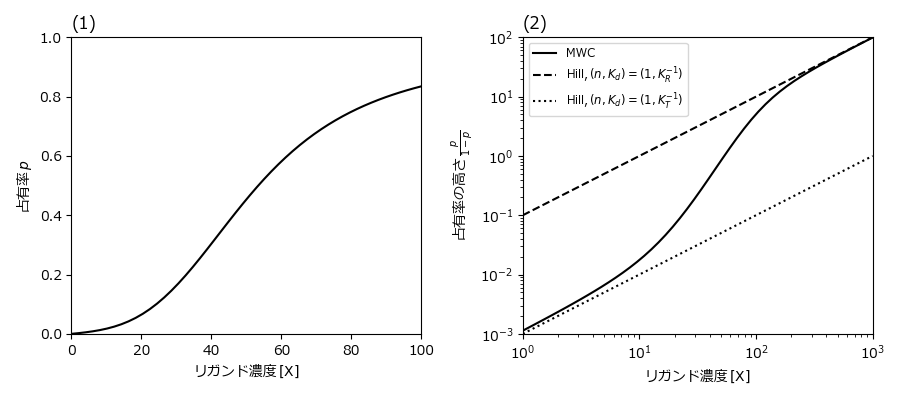
\includegraphics[width=14cm]{mwc.png}
  \caption{(1)MWCモデルによって得られる曲線($n = 4,\, K_{\ce{R}} = 0.1,\, L_0 = 1000,\, c = 0.01$)と(2)そのHillプロット(実線)および会合定数$K_{\ce{R}},K_{\ce{T}}$に対応する$n=1$のHillプロット(それぞれ破線,点線)}
  \label{fig:mwc}
\end{figure}

\subsection{Hillプロット}
MWCモデルで得られる曲線は,一般にHillプロットで直線にならず(図\ref{fig:mwc}(2)),ヘモグロビンと酸素の結合をうまく記述できることが知られている\footnote{ヘモグロビンは4量体なので$n=4$とすれば記述できる.}.
また図\ref{fig:mwc}(2)を見ると,MWCモデルのHillプロットはリガンド濃度が大きい極限と小さい極限で直線に漸近することが分かる.
ここではその理由と漸近線の意味を考える\footnote{この節では参考文献\cite{TBoC}の内容ではなく,私の考察を書いた.}.

まず,式\eqref{mwc}より
\begin{equation}
  \frac{p}{1-p} = x\frac{(1+x)^{n-1} + L_0 c(1+cx)^{n-1}}{(1+x)^{n-1} + L_0 (1+cx)^{n-1}} = x\frac{1+L_0c\qty(\frac{1+cx}{1+x})^{n-1}}{1+L_0\qty(\frac{1+cx}{1+x})^{n-1}}
\end{equation}
が分かる.
ここで$[\ce{X}] \ll 1$のとき$x \ll 1$であり,このとき
\begin{equation}
  \qty(\frac{1+cx}{1+x})^{n-1} \approx 1
\end{equation}
なので
\begin{equation}
  \frac{p}{1-p} \approx x\frac{1+L_0c}{1+L_0}
\end{equation}
がいえる.
さらに式\eqref{ggll}より,$1 \ll Lc  \ll L$であることを考えると,これはさらに
\begin{equation}
  \frac{p}{1-p} \approx cx = K_{\ce{T}}[\ce{X}] 
\end{equation}
と近似できる.
したがって
\begin{equation}
  \log{\frac{p}{1-p}} \approx  \log{[\ce{X}]} + \log{K_{\ce{T}}} \label{hill_t}
\end{equation}
となる.
つまり$[\ce{X}] \ll 1$でHillプロットは傾き1の直線になる.
さらに言えば,これはHillの式で$n=1,\,K_d=K_{\ce{T}}^{-1}$のときに対応する\footnote{$K_{\ce{T}}$は会合定数なので,その逆数$K_{\ce{T}}^{-1}$は解離定数を意味する.}.
よって,これはT状態の一段階反応に対応している.
物理的には,リガンドが少ない状況においてリガンドと受容体の反応はほぼ$\ce{T_0 + X <=> T_1}$が占めると解釈できる.

一方で$[\ce{X}] \gg 1$のとき$x \gg 1$であり,このとき
\begin{equation}
  \qty(\frac{1+cx}{1+x})^{n-1} \approx c
\end{equation}
なので
\begin{equation}
  \frac{p}{1-p} \approx x\frac{1+L_0c^n}{1+L_0c^{n-1}}
\end{equation}
がいえる.
さらに式\eqref{ggll}と式\eqref{ng}より,$n\ge 4$に対しては$1 \gg L_0c^{n-1}  \gg L_0c^{n}$である\footnote{式\eqref{ng}は$L_0c^2$が1と同程度かそれ未満のスケールであることを意味する.ここに$c$をかけると式\eqref{ggll}から$L_0 c^3 \ll 1$がいえるので,一般に$n\ge 4$に対して$1 \gg L_0 c^{n-1} \gg L_0 c^{n}$が成り立つ.もし$L_0c^2$が1未満のスケールなら$n=3$でも成り立ち,$L_0c$が1未満のスケールなら$n=2$でも成り立つ.}ことを考えると,$n \ge 4$のときこれはさらに
\begin{equation}
  \frac{p}{1-p} \approx x = K_{\ce{R}}[\ce{X}] 
\end{equation}
と近似できる.
したがって
\begin{equation}
  \log{\frac{p}{1-p}} \approx  \log{[\ce{X}]} + \log{K_{\ce{R}}} \label{hill_r}
\end{equation}
となる.
つまり$[\ce{X}] \gg 1$でもHillプロットは傾き1の直線になる.
さらに言えば,$n \ge 4$のときこれはHillの式で$n=1,\,K_d=K_{\ce{R}}^{-1}$のときに対応する.
よって,これはR状態の一段階反応に対応している.
物理的には,リガンドが多い状況においてリガンドと受容体の反応はほぼ$\ce{R_{$n-1$} + X <=> R_{$n$}}$が占めると解釈できる.

\subsection{応用}
MWCモデルが当てはまる例はヘモグロビンと酸素の結合以外にも確認されている.
有名な例としてバクテリアが挙げられる.
バクテリアは自分の栄養になる物質などの誘引物質を感知し,その濃度が高い方へ運動する.
これは走化性と呼ばれ,誘引物質が受容体に結合したことで発されるシグナルに応答することで実現している.
この誘引物質と受容体の結合も,MWCモデルがよく当てはまることが知られる.